\section{Activities}
\label{sec:Activities}
%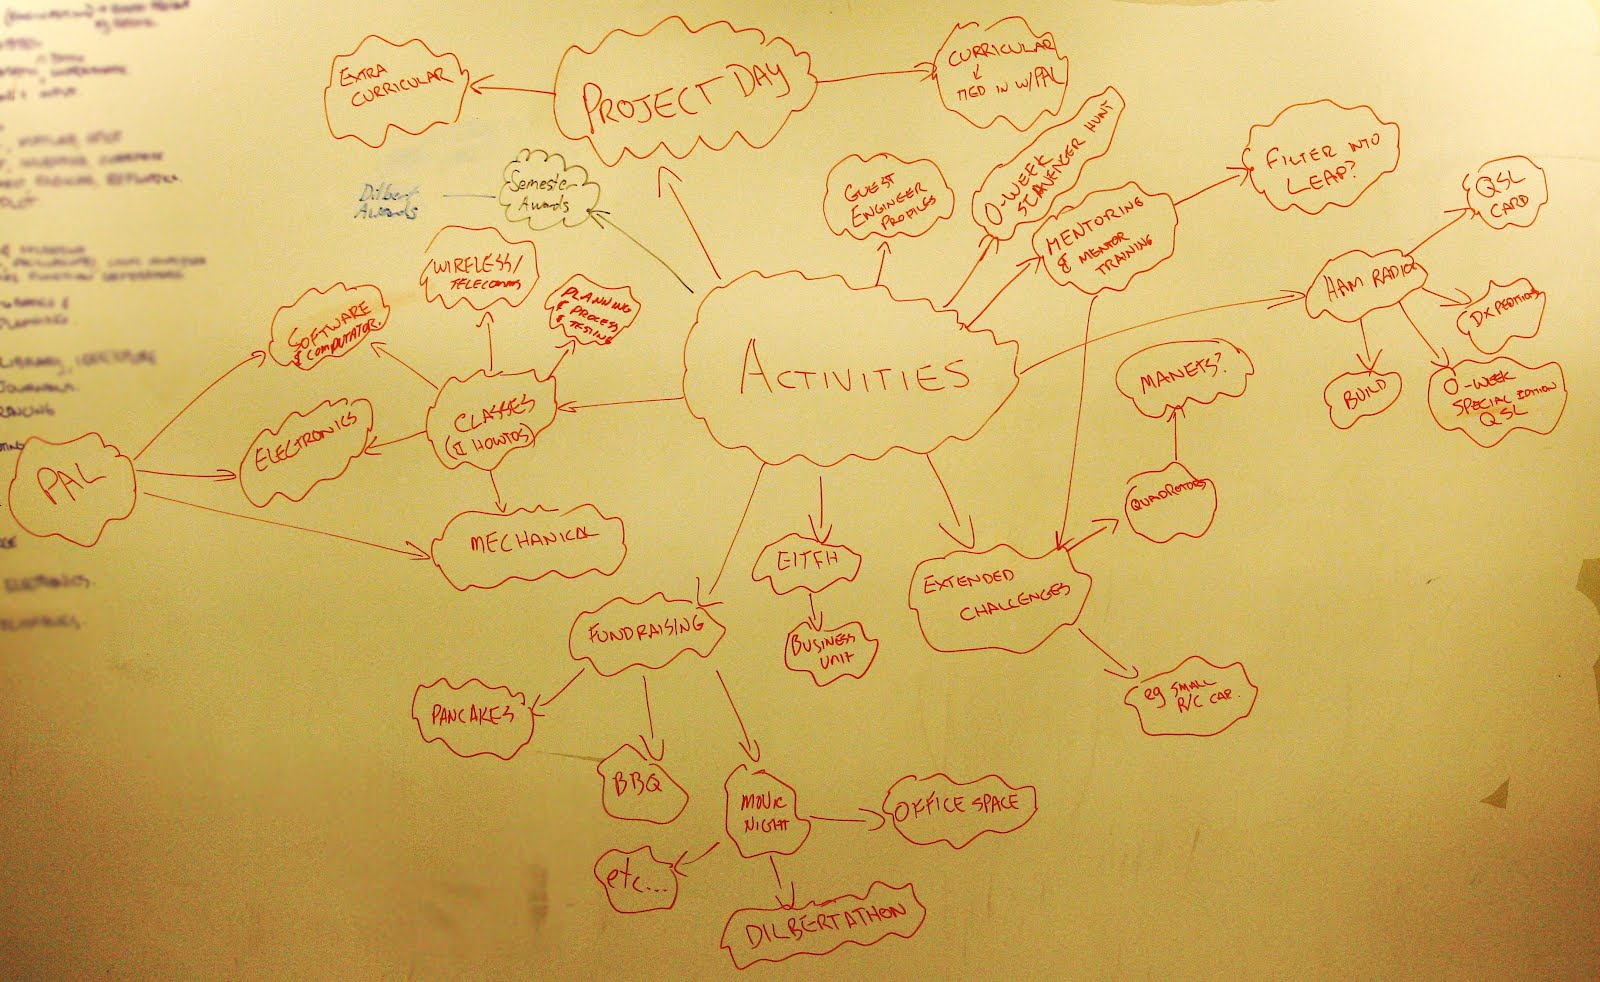
\includegraphics[angle=90, scale=0.18]{img/activities.jpg}
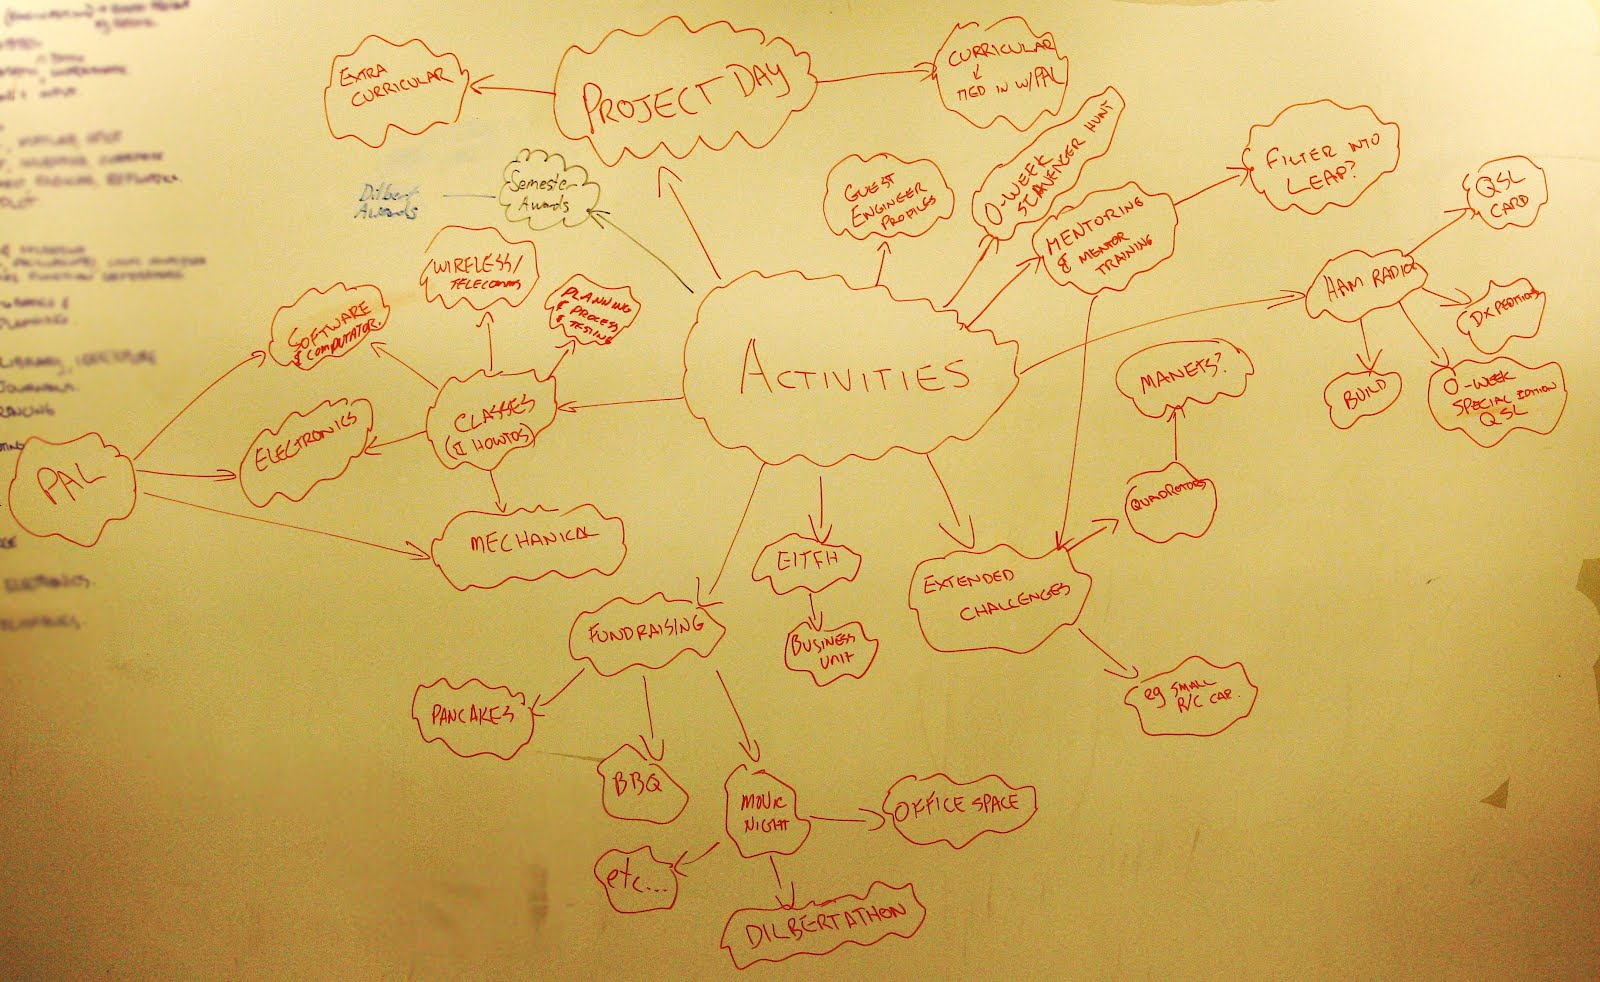
\includegraphics[angle=90, height=\textheight]{img/activities.jpg}
\subsection{Outcome}
While the possible activities is large and varied, we have identified the
following core areas:
\begin{itemize}
  \item Guest Lecturers (possibly professional engineer profiles)
  \item Classes (seminars and workshops)
  \item Project Days
  \item PAL
  \item Fundraisers
  \item Mentoring
  \item Amateur Radio
  \item Social Get togethers (Weekly)
  \item Start of year Engineering Induction with Dept of Engineering
  \item End of Semester Event (with awards)
  \item TEDx Macquarie
\end{itemize}

\subsubsection{Classes}
Classes are a large area of involvement where we would run lectures, seminars
and workshops on areas of interest, some of these are as follows:
\begin{itemize}
  \item Presentation - how to present yourself (eg resume, give talks etc)
  \item \LaTeX and BiBTeX
  \item Maths workshops geared towards engineering. (Need Mike's input)
  \item Software Tools
  \begin{itemize}
    \item AWR
    \item MATLAB
    \item SPICE
    \item OPNET
    \item Inventor
    \item Enterprise Architect
    \item EndNote
    \item Refworks
    \item GNUPLOT
  \end{itemize}
  \item UML
  \item Lab Equipment
  \begin{itemize}
    \item Use of equipment
    \item Soldering
    \item Multimeter
    \item Oscilloscopes
    \item Logic Analyser
    \item Power Supplied
    \item Function Generator
  \end{itemize}
  \item Engineering Logbooks, processes and planning (howtos)
  \item How to use resources (eg library, IEEEXplore, Journals)
  \item How to do referencing properly
  \item Embedded Computing
  \begin{itemize}
    \item Introduction (eg Arduino)
    \item Feedback Controls
  \end{itemize}
  \item EWB Challenge
  \item Funway Into Electronics
  \item Exam Preparation Techniques
\end{itemize}

\subsubsection{Social}
Social activities are also widely varied. Some options open to us:
\begin{itemize}
  \item Weekly meeting at the bar or coffee shop.
  \item Pancake / BBQ
  \item Movie Night
  \item Amateur Radio Days (in association with MQARC)
\end{itemize}

\subsubsection{PAL}
PAL (Peer Assisted Learning) is an initiative that Mike Heimlich has tried to
promote where by students assist each other in learning about engineering. It
has predominantly focused on maths, however there is no reason it cannot broaden
itself to general engineering principles such as use of lab equipment,
whiteboards, and desk space.

It would provide a place for learning through open exploration of ideas with
peers.